\documentclass[12pt]{report}
%\documentclass[titlepage, a4paper, 12pt, reqno, openany]{report}
%\documentclass[12pt]{article}

%%%%%%%%%%%%%%%%%%%%%%%%%%%%%%%%%%%%%%%%%%%%%%%%%%%%%%%%%%%%%%%%%%%%%%%%%%%%%
%%%%%%encoding%%%%%%
\usepackage[T1]{fontenc}
\usepackage{times}
\usepackage[utf8]{inputenc}
%%%%Portuguese-specific commands
\usepackage[portuguese]{babel}
%%%%%%Hyphenation rules%%%%%%
\usepackage{hyphenat}
\usepackage{babelbib}
\usepackage{amsfonts}
\usepackage[top=2cm,left=1.5cm,right=1.5cm,bottom=1.5cm]{geometry} %margens
\usepackage{graphicx} %permite inserir figuras
\usepackage{float}
\usepackage{amsmath}
\usepackage{amssymb}
\usepackage{makeidx} %pra criar índice remissivo
%%%%%%%%%%%%%%%%%%%%%%%%%%%%%%%%%%%%%%%%%%%%%%%%%%%%%%%%%%%%%%%%%%%%%%%%%%%%%%%
\usepackage{babel}
\usepackage{array}
\usepackage{supertabular}
\usepackage{color,colortbl,multirow}
\usepackage{bm}
\usepackage{booktabs}
\usepackage{boxedminipage}
\usepackage{caption}
\usepackage{changepage}
\usepackage{cite}
\usepackage{easylist}
\usepackage{esint}
\usepackage{eucal}
\usepackage{fancyhdr}
%\usepackage{hyperref} %index dentro de red boxes
\usepackage{indentfirst}
\usepackage{latexsym}
\usepackage{listings}
\usepackage{mathptmx}
\usepackage{mathrsfs} %permite o uso de letras trabalhadas
\usepackage{microtype}
\usepackage{multicol}
\usepackage[normalem]{ulem} %permite sublinhar palavras
\usepackage{paralist}
\usepackage{pifont}
\usepackage{rotating}
\usepackage{setspace}
\usepackage{syntonly} %speedup work desabling pdf converse \syntaxonly
\usepackage{subfiles}
\usepackage{subcaption}
\usepackage{textcomp}
\usepackage{theorem}
\usepackage{ulem}
\usepackage{url}
\usepackage{verbatim}
\usepackage{wrapfig}
%%%%%recent%%%%%
\usepackage{cancel}
\usepackage[fleqn]{mathtools}
\usepackage{pdfpages}
\usepackage{pdflscape}
\usepackage{todonotes}
\usepackage{siunitx}
%%%%%%%%%%%%%%%%%%%%%%%%%%%%%%%%%%%%%%%%%%%%%%%%%%%%%%%%%%%%%%%%%%%%%%%%%%%%%%%%%%%
%\renewcommand\thesection{\arabic{section}}
%\renewcommand\thesubsection{\thesection.\arabic{subsection}}
%%%%%%%%%%%%%%%%%%%%%%%%%%%%%%%%%%%%%%%%%%%%%%%%%%%%%%%%%%%%%%%%%%%%%%%%%%%%%%%%%%%%
\usepackage{enumitem}
\begin{comment}
\setlistdepth{12}
\newlist{enumitem}{enumerate}{12}
\setlist[enumitem,1]{label=\roman*)}
\setlist[enumitem,2]{label=\alph*)}
\setlist[enumitem,3]{label=\arabic*)}
\setlist[enumitem,4]{label=(\roman*)}
\setlist[enumitem,5]{label=(\alph*)}
\setlist[enumitem,6]{label=(\arabic*)}
\setlist[enumitem,7]{label=\roman*)}
\setlist[enumitem,8]{label=\alph*)}
\setlist[enumitem,9]{label=\arabic*)}
\setlist[enumitem,10]{label=(\roman*)}
\setlist[enumitem,11]{label=(\alph*)}
\setlist[enumitem,12]{label=(\arabic*)}
\end{comment}

%%%%%%%%%%%%%%%%%%%%%%%%%%%%%%%%%%%%%%%%%%%%%%%%%%%%%%%%%%%%%%%%%%%%%%%%%%%%%%%%%%%%
\usepackage{enumerate}
\begin{comment}
\renewcommand{\labelitemi}{$\bullet$}
\renewcommand{\labelitemii}{$\cdot$}
\renewcommand{\labelitemiii}{$\diamond$}
\renewcommand{\labelitemiv}{$\ast$}
\end{comment}

%%%%%%%%%%%%%%%%%%%%%%%%%%%%%%%%%%%%%%%%%%%%%%%%%%%%%%%%%%%%%%%%%%%%%%%%%%%%%%%%%%%%
\usepackage{tikz}
\usepackage{circuitikz}
\usetikzlibrary{matrix,shapes.geometric,arrows,trees,positioning,calc}
\begin{comment}
\tikzstyle{RECTANGLE_2} = [rectangle, draw, text width=5em, text centered, rounded corners, minimum height=4em]
\tikzstyle{RECTANGLE_3} = [rectangle, rounded corners, minimum width=3cm, minimum height=1cm,text centered, draw=black, fill=red!80]
\tikzstyle{RECTANGLE_4} = [rectangle, draw, fill=blue!20, text width=3cm, text centered, minimum height=4em]
\tikzstyle{RECTANGLE_5} = [rectangle, minimum width=3cm, minimum height=1cm, text centered, text width=3cm]
\tikzstyle{RECTANGLE_6} = [rectangle, draw, fill=blue!20, text width=5em, text centered, rounded corners, minimum height=4em]
\tikzstyle{RECTANGLE_7} = [rectangle, draw, fill=blue!20, text width=5em, text centered, rounded corners, minimum height=4em]
\tikzstyle{RECTANGLE_8} = [rectangle, draw, align=left, fill=blue!20]
\tikzstyle{RECTANGLE_1} = [rectangle, rounded corners, minimum width=1cm, minimum height=1cm,text centered, draw=black, fill=green!%30]
\tikzstyle{DIAMOND_1} = [diamond, draw, fill=blue!20, text width=4.5em, text badly centered, node distance=4cm, inner sep=0pt]
\tikzstyle{DIAMOND_2} = [diamond, minimum width=3cm, minimum height=1cm, text centered, draw=black, fill=green!30]
\tikzstyle{DIAMOND_3} = [diamond, draw, text width=4.5em, text badly centered, node distance=3cm, inner sep=0pt]
\tikzstyle{DIAMOND_4} = [diamond, draw, fill=blue!20, text width=4.5em, text badly centered, node distance=3cm, inner sep=0pt]
\tikzstyle{DIAMOND_5} = [diamond, draw, fill=blue!20, text width=4.5em, text badly centered, node distance=3cm, inner sep=0pt]
\tikzstyle{DIAMOND_6} = [diamond, draw, fill=blue!20, text width=4.5em, text badly centered, node distance=4cm, inner sep=0pt]
\tikzstyle{DIAMOND_7} = [diamond, draw, align=left, fill=blue!20]
\tikzstyle{ELLIPSE_1} = [draw, ellipse,fill=red!20, node distance=3cm, minimum height=2em]
\tikzstyle{ELLIPSE_2} = [draw, ellipse,fill=red!20, node distance=3cm, minimum height=2em]
\tikzstyle{ELLIPSE} = [draw, ellipse,fill=red!20, node distance=3cm, minimum height=2em]
\tikzstyle{TRAPEZIUM_1} = [trapezium,trapezium left angle=70,trapezium right angle=-70,minimum height=0.6cm, draw, fill=blue!20, text width=4.5em, text badly centered, node distance=3cm, inner sep=0pt]
\tikzstyle{TRAPEZIUM_2} = [trapezium, trapezium left angle=70, trapezium right angle=110, minimum width=3cm, minimum height=1cm, text centered, draw=black, fill=blue!30]
\tikzstyle{TRAPEZIUM_3} = [trapezium,trapezium left angle=70,trapezium right angle=-70,minimum height=0.6cm, draw, fill=blue!20, text width=4.5em, text badly centered, node distance=3cm, inner sep=0pt]
\tikzstyle{ARROW} = [thick,->,>=stealth]
\tikzstyle{LINE} = [draw, -latex']
\tikzstyle{MYLINE} = [draw, ->,  thick, shorten <=4pt, shorten >=4pt]
\tikzstyle{TEXT_1}=[draw,text centered,minimum size=6em,text width=5.25cm,text height=0.34cm]
\tikzstyle{TEXT_2}=[draw,text centered,minimum size=2em,text width=2.75cm,text height=0.34cm]
\tikzstyle{TEXT_3}=[draw,minimum size=2.5em,text centered,text width=3.5cm]
\tikzstyle{TEXT_4}=[draw,minimum size=3em,text centered,text width=6.cm]
\tikzstyle{CIRCLE_1}=[draw,shape=circle,inner sep=2pt,text centered, node distance=3.5cm]
\tikzstyle{CIRCLE_2}=[draw,shape=circle,inner sep=4pt,text centered, node distance=3.cm]
\end{comment}

%%%%%%%%%%%%%%%%%%%%%%%%%%%%%%%%%Not Adviced%%%%%%%%%%%%%%%%%%%%%%%%%%%%%%%%%%%%%%%%
%\usepackage{showidx} %for troubleshooting index
%\usepackage{showkeys} %for troubleshooting \label \ref
%\usepackage{pxfonts}

%%%%%%%%%%%%%%%%%%%%%%%%%%%%%%%%%claching Package%%%%%%%%%%%%%%%%%%%%%%%%%%%%%%%%%%%
%\usepackage[usenames,dvipsnames,svgnames,table]{xcolor} %\usepackage[usenames]{color} %permite letras coloridas
%\usepackage{pgfplots}
%\usepackage{natbib}
%\usepackage[usenames]{color} %permite letras coloridas
%\usepackage{xypic}

%%%%%%%%%%%%%%%%%%%%%%%%%%%%%%%%%Not Installed Yet%%%%%%%%%%%%%%%%%%%%%%%%%%%%%%%%%%

%%%%%%%%%%%%%%%%%%%%%%%%%%%%%%%Com Dependencias%%%%%%%%%%%%%%%%%%%%%%%%%%%%%%%%%%%%%
%\usepackage{glossaries}
%\usepackage[version=3]{mhchem}

%%%%%%%%%%%%%%%%%%%%%%%%%%%%%%%%%%%%%%%%%%%%%%%%%%%%%%%%%%%%%%%%%%%%%%%%%%%%%%%%%%%%
%alguns pacotes nao sao reconhecidos, ter atencao quais usar em differents computadores, tambem alguns pacotes entram em conflito.
\newtheorem{theorem}{Theorem}
\newtheorem{lemma}{Lemma}
\newtheorem{definition}{Defini\c{c}\~{a}o}
\newtheorem{notation}{Notation}

%%%%%%%%%%%%%%%%%%%%%%%%%%%%%%%%Not Working%%%%%%%%%%%%%%%%%%%%%%%%%%%%%%%%%%%%%%%%%
%\usepackage{itemize}
%\usepackage{named}
%\usepackage{amscls}
%\usepackage{fullpage}

%%%%%%%%%%%%%%%%%%%%%%%%%%%%%%%%%%%%%%%%%%%%%%%%%%%%%%%%%%%%%%%%%%%%%%%%%%%%%%%%%%%%
\makeindex
\bibliographystyle{babplain}
\begin{document}

%
\begin{titlepage}
\begin{minipage}{0.95\linewidth}
\centering

\includegraphics[scale=0.60]{./image/capa/ISEP_marca_cor_grande.png}
\label{Capa}
\title{Estatística}
\author{
\emph{S\'{e}rgio Manuel Salazar dos Santos},\;$N^o$:\; 1020881 \\
%\emph{Nome 2},\;$N^o$:\; 2000000\\
%\emph{Nome 3},\;$N^o$:\; 3000000\\
%\emph{Nome 4},\;$N^o$:\; 4000000\\
%\emph{Nome 5},\;$N^o$:\; 5000000\\
}
\date{\today}
\maketitle
\end{minipage}
\end{titlepage}
%
\tableofcontents
%
\appendix
%
\pagestyle{plain}%plain headings empty
%%%%%%%%%%%%%%%%%%%%%%%%%%%%%%%%%%%%%%%%%%%%
\newpage
\label{Resumo}
\begin{abstract}
Este trabalho consiste no estudo de Estatística das Entregas Expresso em  duas regiões \textbf{A} e \textbf{B}, as variaveis em estudo é o tempo de demora das entregas e a variavel de numero de encomendas entregues num determinado unidade de tempo [u.t.]. Nestas situações foram retiradas 120 e 90 amostras nas duas regiões respectivamente.\\
A primeira é uma distribuição continua, o tempo, e a segunda uma distribuição discreta.
\\
As materias abordadas vai ser \textbf{Amostragem}, \textbf{Estimação de parâmetros} e \textbf{Testes de Hipóteses}\\
\end{abstract}
%
\newpage
\section{Introdução}\label{Introdução}
%
As variáveis consideradas são:
\begin{itemize}
\item[$-$] Regiao (REG): variável nominal com dois niveis\\
\qquad Regiao A \\
\qquad Região B
\item [$-$] Tempo de entrega (TEE), por encomenda: Variável expressa em u.t.
\item [$-$] Número de encomendas entregues (NEE) por u.t.
\end{itemize}
Admitindo que a amostra disponível é uma amostra aleatória representativa das populações.\\
\\
Neste relatorio esta-se a trabalhar com duas  grandezas precisamente o tempo (TEE) e quantidade por u.t (NEE), temos recolhidos 120 registos \textbf{TEE} na qual pela regra de sturges $c = int(1+3.3log(n))$, determina-se que é necesario sete [\textbf{7}] classes. \\
Podemos obter a amplitude de cada classe $h=b-a$ e sua marca $x_i=\frac{a+b}{2}$. \\
\section{O conjunto de dados}\label{dados}
\noindent
$X_{i_A}$- "Variavel aleatoria que representa o tempo de demora na Região \textbf{A} da entrega de uma encomenda Expresso em u.t." \quad i=1,2,3, .....,120 \\
$X_{i_B}$- "Variavel aleatoria que representa o tempo de demora na Região \textbf{B} da entrega de uma encomenda Expresso em u.t." \quad i=1,2,3, .....,120 \\
Abaixo o resultado da tabela TEE:\\
\\
\begin{minipage}{0pt}
\begin{tabular}{ |c|c|c|c|c|c|c|c|c|c|c| }
\hline
$h_i$ & CLASSE & MARCA & $n_{i_A}$ & $n_{i_B}$ & $\frac{n_{i_A}}{h_i}$ & $\frac{n_{i_B}}{h_i}$ & $f_{i_A}$	& $f_{i_B}$ & $F_{i_A}$ & $F_{i_B}$ \\
\hline
4 & [5,10[ & 7,5 & 8 & 1 & 2 & 0,25 & 0,0667 & 0,0083 & 0,0667 & 0,0083 \\
\hline
4 & [10,15[ & 12,5 & 16 & 18 & 4 & 4,5 & 0,1333 & 0,15 & 0,2 & 0,1583 \\
\hline
4 & [15,20[ & 17,5 & 40 & 28 & 10 & 7 & 0,3333 & 0,2333 & 0,5333 & 0,3917 \\
\hline
4 & [20,25[ & 22,5 & 25 & 41 & 6,25 & 10,25 & 0,2083 & 0,3417 & 0,7417 & 0,7333 \\
\hline
4 & [25,30[ & 27,5 & 26 & 22 & 6,5 & 5,5 & 0,2167 & 0,1833 & 0,9583 & 0,9167 \\
\hline
4 & [30,35[ & 32,5 & 4 & 8 & 1 & 2 & 0,0333 & 0,0667 & 0,9917 & 0,9833 \\
\hline
5 & [35,40] & 37,5 & 1 & 2 & 0,2 & 0,4 & 0,0083 & 0,0167 & 1 & 1 \\
\hline
& & & n=120 & n=120 & & & & & & \\
\hline
\end{tabular}
\end{minipage}
\\
$n_i$ - frequência absoluta
$f_i$ - frequência relativa
$F_i$ - frequência acumulada
\\
\\
Recorrendo ao excell obeteve-se os seguintes resultados: \\
\begin{minipage}{0pt}
$$\begin{array}{l | l}
\text{Média aritmetica dados classificados} & \text{Variância de uma amostra dados classificados} \\
\overline{x} = \frac{1}{n}\sum_{i=1}^cx_in_i = \sum_{i=1}^cx_if_i & s^2 = \frac{1}{n-1}\sum_{i=1}^c (x_i-\bar{x})^2 n_i
\end{array}$$
\end{minipage}
\\
\begin{minipage}[!b]{0.40\linewidth}
\begin{tabular}{ l c c }
\hline
Estatística & $X_A$ & $X_B$ \\
\hline
Mínimo & 7,5 & 7,5\\
$Q_1$:$1^o$ Quartil & 17,5 & 17,5 \\
$m_d$: mediana & 17,5 & 22,5\\
$Q_3$:$3^o$ Quartil & 27,5 & 27,5 \\
Máximo & 37,5 & 37,5 \\
\hline
$\bar{X}$ : Média & 20,0417 & 21,5417 \\
$s$ : desvio-padrão & 6,4494 & 6,0909\\
$m_o$: moda & 17,5 & 22,5\\
\hline
Tamanho amostral [$n$] & 120 & 120 \\
\hline
\end{tabular}
\label{Tab:Resulatdos}
\end{minipage}
\hspace{2cm}
\begin{minipage}[!b]{0.40\linewidth}
\begin{figure}[H]
\centering
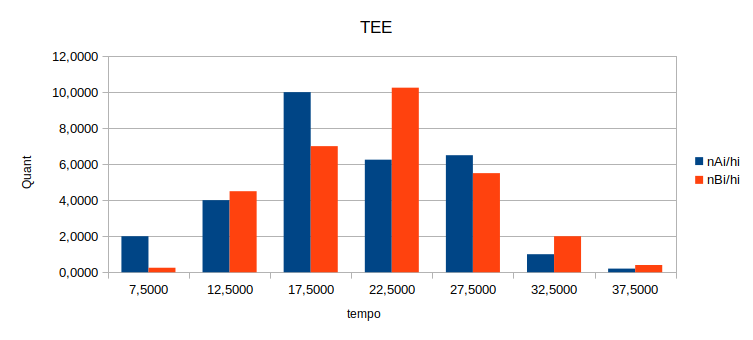
\includegraphics[scale=0.5]{./image/TEE.png}
\caption{TEE}
\label{TEE}
\end{figure}
\end{minipage}
\\
\\
\\
\noindent
A mediana pode ser obtida pela frequencia acumulativa quando esta é igual a 50\%, ou seja, $F_i(Mediana)=0,5$ \\
\\
Linearização mediana \textbf{TEE}\\
\\
\begin{minipage}[l]{0pt}
\begin{tabular}{l}
Regiao \textbf{A}:\\
0.2 $\implies$ 12.5 \\
0.5333 $\implies$ 17.5 \\
$\therefore$\\
Midiana A = \\
12.5 + 0.9 x (17.5-12.5) = 17 \\
com: \\
skew = -0,1051 e kurt = -0,4016 \\
\end{tabular}
\end{minipage} \hspace{10cm}
\begin{minipage}[l]{0pt}
\begin{tabular}{l}
Regiao \textbf{B}: \\
0.3917 $\implies$ 17.5 \\
0.7333 $\implies$ 22.5 \\
$\therefore$\\
Midiana B = \\
17.5 + 0.317 x (22.5-17.5) = 19.085 \\
com : \\
skew = 0,1119 e kurt = -0,1835 \\
\end{tabular}
\end{minipage}\\
\\
\\
\noindent
Na prática, considera-se que a qualidade da aproximação é suficientemente boa quando $n \geqslant 30$.  \\
Pode-se tomar que $\delta \cong s$. \\
\begin{minipage}[l]{0pt}
$$\left\lbrace\begin{array}{c}
\mu \\
\delta \\
\end{array}\right.$$
\end{minipage}
\hspace{3cm} $\Longrightarrow$ \hspace{3cm}
\begin{minipage}[l]{0pt}
\[\bar{X}=\frac{\sum_{i=1}^nX_i}{n}\sim N \big(\mu;\frac{\delta^2}{n}\big)\]
\end{minipage}\\
\\
$\bar{x}_{A_0}$ = 20,0417 \qquad $\bar{x}_{B_0}$ = 21,5417 \\
$\delta_A$ = 6,4494 \qquad $\delta_B$ = 6,0909\\
\\
\\
%%%%%%%%%%%%%%%%%%%%%%%%%%%%%%%%%%%%%%%%%%%%%%%%%%%%%%%%%%%%%%%%%%%%%%%%%%%%%%%%%%%%
\noindent
Tratamento dos dados da Segunda Variavel Aleatótia \\
$Y_{i_A}$- "Variavel aleatoria que representa o numero de encomendas entregues pela Expresso na Regiao \textbf{A} por u.t." \quad i=1,2,3, .....,90 \\
$Y_{i_B}$- "Variavel aleatoria que representa a numero de encomendas entregues pela Expresso na Regiao \textbf{B} por u.t." \quad i=1,2,3, .....,90 \\
Abaixo o resultado da tabela NEE:\\
\\
\begin{minipage}{0pt}
\begin{tabular}{ |c|c|c|c|c|c|c| }
\hline
$Y_i$ & $n_{i_A}$ & $n_{i_B}$ & $f_{i_A}$ & $f_{i_B}$ & $F_{i_A}$ & $F_{i_B}$ \\
\hline
3 & 6 & 3 & 0,0667 & 0,0333 & 0,0667 & 0,0333 \\
\hline
4 & 8 & 6 & 0,0889 & 0,0667 & 0,1556 & 0,1 \\
\hline
5 & 19 & 13 & 0,2111 & 0,1444 & 0,3677 & 0,2444 \\
\hline
6 & 15 & 7 & 0,1667 & 0,0778 & 0,5333 & 0,3222 \\
\hline
7 & 13 & 19 & 0,1444 & 0,2111 & 0,6778 & 0,5333 \\
\hline
8 & 11 & 15 & 0,1222 & 0,1667 & 0,8 & 0,7 \\
\hline
9 & 6 & 8 & 0,0667 & 0,0889 & 0,8667 & 0,7889 \\
\hline
10 & 5 & 11 & 0,0556 & 0,1222 & 0,9222 & 0,9111 \\
\hline
11 & 4 & 3 & 0,0444 & 0,0333 & 0,9667 & 0,9444 \\
\hline
12 & 0 & 2 & 0 & 0,0222 & 0,9667 & 0,9667 \\
\hline
13 & 2 & 1 & 0,0222 & 0,0111 & 0,9889 & 0.9778 \\
\hline
14 & 1 & 0 & 0,0111 & 0 & 1 & 0,9778 \\
\hline
15 & 0 & 1 & 0 & 0,0111 & 1 & 0,9889 \\
\hline
16 & 0 & 1 & 0 & 0,0111 & 1 & 1 \\
\hline
\end{tabular}
\end{minipage}
\\
\begin{minipage}[!b]{0.40\linewidth}
\begin{tabular}{ l c c }
\hline
Estatística & $Y_A$ & $Y_B$ \\
\hline
Mínimo & 3 & 3 \\
$Q_1$:$1^o$ Quartil & 5 & 6 \\
$m_d$: mediana & 6 & 7 \\
$Q_3$:$3^o$ Quartil & 8 & 9 \\
Máximo & 14 & 16 \\
\hline
$\bar{Y}$ : Média & 6,6111 & 7,5111 \\
$s$ : desvio-padrão & 2,3112 & 2,5140\\
$m_o$: moda & 5 & 7\\
\hline
Tamanho amostral [$n$] & 90 & 90 \\
\hline
\end{tabular}
\label{Tab:Resulatdos}
\end{minipage}
\hspace{1.8cm}
\begin{minipage}[!b]{0.40\linewidth}
\begin{figure}[H]
\centering
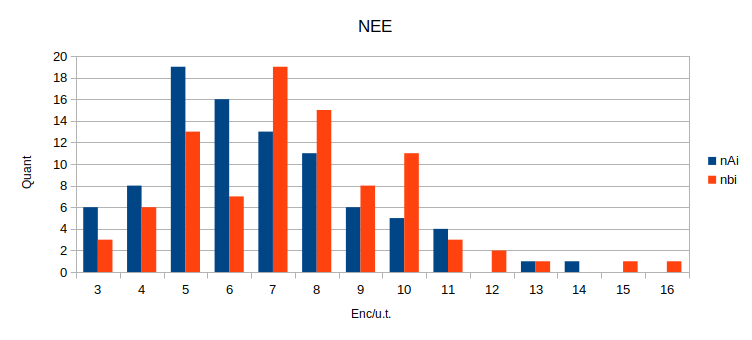
\includegraphics[scale=0.5]{./image/NEE.png}
\caption{NEE}
\label{NEE}
\end{figure}
\end{minipage}
\\
\\
\noindent
Na Região \textbf{A} a Média > Mediana > Moda \\ 
com skew = 0.74553  e kurt = 0.49789 \\
Na Região \textbf{B} a Média > Mediana = Moda \\
com skew = 0.67659 e kurt = 1.01076 \\
\begin{minipage}[l]{0pt}
$$\left\lbrace\begin{array}{c}
\mu \\
\delta \\
\end{array}\right.$$
\end{minipage}
\hspace{3cm} $\Longrightarrow$ \hspace{3cm}
\begin{minipage}[l]{0pt}
\[\bar{Y}=\frac{\sum_{i=1}^nY_i}{n}\sim N \big(\mu;\frac{\delta^2}{n}\big)\]
\end{minipage}\\
\\
$\bar{y}_{A_0}$ = 6,6111 \qquad $\bar{y}_{B_0}$ = 7,5111 \\
$\delta_A$ = 2,3112 \qquad $\delta_B$ = 2,5140 \\
\\
%%%%%%%%%%%%%%%%%%%%%%%%%%%%%%%%%%%%%%%%%%%%%%%%%%%%%%%%%%%%%%%%%%%%%%%%%%%%%%%%%%%%%
\newpage
\section{Metodologia Estatística}\label{Metodos}
\noindent
\subsection{Indice de Confiançã tempo médio TEE}
Estimação do tempo médio para as regiões \textbf{A} e \textbf{B} com um indice de confiança de 95\%. \\
\\
$IC_{1-\alpha}=\left[ A, B\right]$ ; para $1-\alpha = 0.95$, $\alpha=0.05$, $\frac{\alpha}{2}=0.025$ \\
Zona critica $Z_c=Z_{1-\frac{\alpha}{2}}=\Phi^{-1}(0.975) \cong 1.96$ \\
$P\left( A \leqslant \mu \leqslant B \right) = 1-\alpha$ \\
$\triangle=Z_c\times\frac{\delta}{\sqrt{n}}$ \\
$A = \bar{x}-\triangle \qquad and \qquad B = \bar{x}+\triangle$ \\
$\therefore$\\
$IC_{A_{0.95}}=\left[ \; 18.8877 \: , \: 21.1956 \; \right]$ \hspace{1cm} and \hspace{1cm} $IC_{B_{0.95}}=\left[ \; 20.4519 \: , \: 22.6314 \; \right]$\\
\\
\noindent
Pode-se estimar que o tempo médio $\left[ \; \mu \; \right]$ de entrega na população  esta dentro dos intervalos acima mencionados com 95\% de confiança.\\
\subsection{Verificar diferença de valores num intervalo}
\noindent
Verificar se os dados permitem afirmar que existe diferença significativa entre a \% de períodos com menos de \textbf{6} entregas por u.t. na região \textbf{A} e na região \textbf{B}. Responda com base num intervalo de confiança de 97\%. \\
\\
Destribuição discreta: \\
\\
$\bar{y}_{A_0}$ = 6,6111 \qquad $\bar{y}_{B_0}$ = 7,5111 \qquad $n=90$ \\
$\delta_A$ = 2,3112 \qquad $\delta_B$ = 2,5140 \\
\begin{minipage}[l]{0pt}
$$\left\lbrace\begin{array}{c}
\mu \\
\delta \\
\end{array}\right.$$
\end{minipage}
\hspace{3cm} $\Longrightarrow$ \hspace{3cm}
\begin{minipage}[l]{0pt}
\[\bar{Y}=\frac{\sum_{i=1}^nY_i}{n}\sim N \big(\mu;\frac{\delta^2}{n}\big)\]
\end{minipage}\\
\\
\\
$P(Y_A < 6)=P(Y_A \leqslant 5)=F_{i_B}(5) \cong 0,3677 $  \quad e \quad $P(Y_B < 6)=P(Y_B \leqslant 5)=F_{i_B}(5) \cong 0,2444$ \\
\\
$\hat{P_A}-\hat{P_B} \sim N \left( p_A - p_B ; \frac{p_A\:q_A}{n_A} + \frac{p_B\:q_B}{n_B}\right)$ \hspace{1cm}
$\triangle=z_{(1-\frac{\alpha}{2})} \;\sqrt{\frac{\hat{p_A} \: \hat{q_A}}{n_A}+\frac{\hat{p_B} \: \hat{q_B}}{n_B}}$ \hspace{1cm} $q=(1-p)$ \\
\\
$IC_{97\%}(\hat{P_A}-\hat{P_B})=\left[(\hat{p_A}-\hat{p_B})-\triangle \: ; \: (\hat{p_A}-\hat{p_B})+\triangle \right]$ \\
\\
$\hat{P_A}-\hat{P_B} \sim N \left( 0,1233 \; ; \; 0,02788\right)$ \hspace{1cm}
$z_{(1-\frac{\alpha}{2})}=\phi^{-1}(0,985)=2,1701$ \\
\\
Recorrendo a calculadaora casio $fx-9860GII$ : \\
\\
$\triangle= InvNorm(0.985)\sqrt{\frac{0.3677(1-0.3677)}{90}+\frac{0.2444(1-0.2444)}{90}}\: \cong \:0.3677$
\\
$\therefore$
\\
$IC_{97\%}(\hat{P_A}-\hat{P_B})=\left[ \; (\hat{p_A}-\hat{p_B}) \:-\: 0,3624 \: ; \: (\hat{p_A}-\hat{p_B}) \:+\: 0,3624 \; \right]$ \\
\\
A Diferença de proporçôes é 36,24\%. \\
\subsection{Verificar diferenças entre as regiões}
\noindent
Testar se a região (REG) tem um efeito estatisticamente significativo sobre TEE e NEE ao nível de diferença de médias. Considrere uma significância à sua escolha inferior ou igual a 5\%. Use o critério do valor de prova para fundamentar a decisão.\\
\\
\begin{minipage}[l]{0pt}
$$\left\lbrace\begin{array}{l}
H_0: \quad \mu_A-\mu_B=0 \\
\\
H_1: \quad \mu_A-\mu_B<0
\end{array}\right.$$
\end{minipage}
\\
\\
\\
\hspace*{5cm} \underline{Condição TEE:}\\
\begin{minipage}[l]{0pt}
$$\left\lbrace\begin{array}{c}
\mu \;=\; 0 \\
\delta \;=\; s \\
\end{array}\right.$$
\end{minipage}
\hspace{3cm} $\Longrightarrow$ \hspace{1cm}
\begin{minipage}[l]{0pt}
\[\bar{X_A}-\bar{X_B} \quad \backsim N \left( 0\:,\: \frac{\delta_A^2}{n_A}+\frac{\delta_B^2}{n_B} \right) \]
\end{minipage}\\
\\
$\bar{x}_A-\bar{x_B}=-1.5$ \\
\\
$ \frac{\delta_A^2}{n_A}+\frac{\delta_B^2}{n_B} $ \\
\\
\begin{minipage}[l]{0pt}
\[  z_0\:=\: \frac{\bar{x}_A-\bar{x_B}}{\sqrt{\frac{\delta_A^2}{n_A}+\frac{\delta_B^2}{n_B}}} \qquad
	RC_z \:=\: \left] -\infty,-z_{1-\alpha} \right]  \qquad
	pvalue \:=\: P(Z<z_0) \]
\end{minipage}\\
\\
\\
\hspace*{5cm} \underline{Condição REE:}\\
\begin{minipage}[l]{0pt}
$$\left\lbrace\begin{array}{c}
\mu \;=\; 0 \\
\delta \;=\; s \\
\end{array}\right.$$
\end{minipage}
\hspace{3cm} $\Longrightarrow$ \hspace{1cm}
\begin{minipage}[l]{0pt}
\[\bar{Y_A}-\bar{Y_B} \quad \backsim N \left( 0\:,\: \frac{\delta_A^2}{n_A}+\frac{\delta_B^2}{n_B} \right) \]
\end{minipage}\\
\\
$ \bar{y_A}-\bar{y_B}=-0.9$\\
\\
$ \frac{\delta_A^2}{n_A}+\frac{\delta_B^2}{n_B} $\\
%\hspace{3cm}
\begin{minipage}[l]{0pt}
\[  z_0\:=\: \frac{\bar{y}_A-\bar{y_B}}{\sqrt{\frac{\delta_A^2}{n_A}+\frac{\delta_B^2}{n_B}}} \qquad
 	RC_z=]-\infty,-z_{1-\alpha}] \qquad
 	pvalue=P(Z<z_0) \]
\end{minipage}\\
\\










\newpage
\subsection{Ajuste distribuição teórica à Empirica}
Ajuste uma distribuição teórica à distribuição empírica das variaveis TEE na região A (considerando as classes definidas) e NEE na região B. Verifique a qualidade do ajuste ao nível de 5\%.\\
\\
\hspace*{5cm} \underline{TEE Região A:} \\
\begin{minipage}[l]{0pt}
$$\left\lbrace\begin{array}{l}
H_0: X \backsim N (20.0417\;,\;6.4494^2) \\
\\
H_1: X \nsim N (20.0417\;,\;6.4494^2)
\end{array}\right.$$
\end{minipage}\\
\\
\\
$q_0=\sum_{i=1}^n \frac{(n_i-e_i)^2}{e_i} \;\backsim\; \chi_{(k-p-1)}^2$ \\
\\
\hspace*{5cm} \underline{NEE Região B:} \\
\begin{minipage}[l]{0pt}
$$\left\lbrace\begin{array}{l}
H_0: X \backsim N (7.5111\;,\;2.5140^2) \\
\\
H_1: X \nsim N (7.5111\;,\;2.5140^2)
\end{array}\right.$$
\end{minipage}\\
\\
\\
$q_0=\sum_{i=1}^n \frac{(n_i-e_i)^2}{e_i} \;\backsim\; \chi_{(k-p-1)}^2$ \\









\newpage




\newpage
\section{Resultados e interpretação}\label{Resultados}
fazer tabela só com resultados\\
\section{Conclusões}\label{Conclusão}
A Destribuição normal tem a Média = Mediana = Moda, devido a ter uma destribuição simetrica, quando estamos a analizar valores discretos isto não acontece devido a não ser simetrico podendo ter varios casos diferentes, e quanto menor o numero de amostras da população maior a dificuldade de se poder inferir e estimar valores.

Falar da skew e curt.


%%%%%%%%%%%%%%%%%%%%%%%%%%%%%%%%%%%%%%%%%%%%%%%%%%%%%%%%%%%%%%%%%%%%%%%%%%%%%%%%%%%%%
%\part*{Equa\c{c}\~{o}es} \label{eq}
%
\begin{flushleft}
{\bf Corrente Continua Condi\c{c}\~{o}es \index{Condi\c{c}\~{o}es} iniciais \index{iniciais} nulas \index{nulas}.}\par
\end{flushleft}
 \quad Circuito \index{Circuito} $LC$ em $C.C$:\par
%
\begin{itemize}
\item
$i(t)=\frac{V_{DC}\sqrt{LC}}{L}\quad \sin \left( \frac{t}{\sqrt{LC}}\right)\times u(t)$\par
\item
$V_L(t)=V_{DC}\quad \cos\left(\frac{t}{\sqrt{LC}} \right)\times u(t)$\par
\item
$V_c(t)=V_{DC}\quad \left(1-\cos\left(\frac{t}{\sqrt{LC}} \right) \right)\times u(t)$\par
\item
$\omega_n=\frac{1}{\sqrt{LC}}$\par
\item
$\overline{Z}=\sqrt{(\omega_n L-\frac{1}{\omega_n C})^2}$\par
\item
$\phi_p=\frac{\pi}{2}$\par
porque, $\sin(\omega_n t)= \cos(\omega_n t - \pi/2)$\par
\item
$\tau=\infty$\par
\end{itemize}
%
%%%%%%%%%%%%%%%%%%%%%
\quad Circuito \index{Circuito} $RLC$ em $C.C$:\par
%
\begin{enumerate}
%enum1
\item
Para \quad $C(C R^2-4 L)>0$ \quad (Ra\'{i}zes \index{Ra\'{i}zes} reais \index{reais} diferentes \index{diferentes}) \quad Sobreamortecido \index{Sobreamortecido}.\par
%
\begin{itemize}
\item
$i(t)=\frac{2 V_{DC} C e^{\frac{-tR}{2L}} sinh \left( \frac{t \sqrt{C(CR^2-4L)}}{2CL} \right)}{\sqrt{C(CR^2-RL)}}\times u(t)$\par
\item
$V_R(t)=R\times i(t)$\par
\item
$V_L(t)=L\dfrac{di(t)}{dt}$\par
%
\begin{minipage}{0.95\linewidth}
\makebox[\linewidth]{
\includegraphics[scale=0.75]{./Image/equacoes_1.png}
}
\end{minipage}\par
%
\item
$V_C(t)=\frac{1}{C}\int_0^ti(t)$\par
%
\begin{minipage}{0.95\linewidth}
\makebox[\linewidth]{
\includegraphics[scale=0.75]{./Image/equacoes_2.png}
}
\end{minipage}\par
%
\end{itemize}
%enum2
\item
Para \quad $C(C R^2-4 L)=0$ \quad (Ra\'{i}zes \index{Ra\'{i}zes} iguais \index{iguais})\quad Amortecimento \index{Amortecimento} cr\'{i}tico \index{cr\'{i}tico}.\par
%
\begin{itemize}
\item
$i(t)=\frac{V_{DC}}{L} \quad  t \quad e^{\frac{-R t}{2L}} \times u(t)$\par
\item
$V_R(t)=R\times i(t)$\par
\item
$V_L(t)=L\dfrac{di(t)}{dt}$\par
%
\begin{minipage}{0.95\linewidth}
\makebox[\linewidth]{
\includegraphics[scale=0.75]{./Image/equacoes_3.png}
}
\end{minipage}\par
%
\item
$V_C(t)=\frac{1}{C}\int_0^ti(t)$\par
\begin{minipage}{0.95\linewidth}
\makebox[\linewidth]{
\includegraphics[scale=0.75]{./Image/equacoes_4.png}
}
\end{minipage}\par
%
\end{itemize}
%enum3
\item
Para \quad $C(C R^2-4 L)<0$ \quad (Ra\'{i}zes \index{Ra\'{i}zes} complexas \index{complexas}) \quad Amortecido \index{Amortecido}.\par
%
\begin{itemize}
\item
$i(t)=\frac{2 V_{DC} C e^{\frac{-tR}{2L}} sin \left( \frac{t \sqrt{-C(CR^2-4L)}}{2CL} \right)}{\sqrt{-C(CR^2-4L)}}\times u(t)$\par
\item
$V_R(t)=R\times i(t)$\par
\item
$V_L(t)=L\dfrac{di(t)}{dt}$\par
%
\begin{minipage}{0.95\linewidth}
\makebox[\linewidth]{
\includegraphics[scale=0.75]{./Image/equacoes_5.png}
}
\end{minipage}\par
%
\item
$V_C(t)=\frac{1}{C}\int_0^ti(t)$\par
%
\begin{minipage}{0.95\linewidth}
\makebox[\linewidth]{
\includegraphics[scale=0.75]{./Image/equacoes_6.png}
}
\end{minipage}\par
%
\end{itemize}
\end{enumerate}
%
\begin{itemize}
\item
$| \omega_n |=\sqrt{\frac{4 L-R^2 C}{4 L^2 C}}$\par
\item
%\overrightarrow{Z}
$\overline{Z}=\sqrt{R^2 + (\omega_n L -\frac{1}{\omega_n C})^2}$\par
\item
$\phi_p=\arctan\left(\frac{\omega_n L - \frac{1}{\omega_n C}}{R}\right)$\par
\item
$\tau=\frac{2 L}{R}$\par
\end{itemize}
%%%%%%%%%%%%%%%%%%%%%%%%%%%%%%%%%%%%%%%%%%
\begin{flushleft}
{\bf Corrente \index{Corrente} Alternada condi\c{c}\~{o}es \index{Condi\c{c}\~{o}es} iniciais \index{iniciais} nulas \index{nulas}}.
\end{flushleft}
\quad Circuito \index{Circuito} $RLE$ em $C.A$:\par
\begin{itemize}
\item
$i(t)=C_T\ e^{-\frac{R}{L}t}+\frac{V_{m\acute{a}x}}{\overline{Z}}\sin(\omega t + \alpha - \phi_p)-\frac{E}{R}$\newline
$i(t)=C_T\ e^{-\frac{R}{L}t} + C_1 \cos (\omega t) + C_2 \sin(\omega t)-\frac{E}{R}$
\item
$I(\omega t)=C_T\ e^{-\frac{R}{L \omega}\omega t}+\frac{V_{m\acute{a}x}}{\overline{Z}}\sin(\omega t + \alpha - \phi_p)-\frac{E}{R}$
\item
$\overrightarrow{Z}=R+j\omega L$\\
$\overline{Z}=\sqrt{R^2 + (\omega L)^2}$
\item
$\phi_p=\arctan(\frac{\omega L}{R})$
\item
$C_T=\frac{E}{R}-\frac{V_{m\acute{a}x}}{\overline{Z}}\sin(\alpha - \phi_p)$
\item
$C_T=\frac{V_{m\acute{a}x}}{R^2 + (\omega L)^2}(L \omega \cos(\alpha) - R \sin (\alpha))+\frac{E}{R}$
\item
$C_1=\frac{V_{m\acute{a}x}}{R^2 + (\omega L)^2}(R \sin (\alpha) - L \omega \cos(\alpha))$
\item
$C_2=\frac{V_{m\acute{a}x}}{R^2 + (\omega L)^2}(R \cos (\alpha) + L \omega \sin (\alpha))$
%
\end{itemize}
%%%%%%%%%%%%%%%%%%%%%%%
%\part*{Defini\c{c}\~{o}es} \label{def}
\begin{definition}
Capacit\^{a}ncia
\begin{flalign*}
Q_c(t) =& \int^t i(t) \quad dt & \\
=& Q_c(0^-)+\int_{0^-}^t i(t) \quad dt & \\
V_c(t) =& \frac{Q_c(t)}{C} & \\
=& \frac{1}{C} \quad \int^t i_c(t) \quad dt & \\
=& \frac{Q_c(0^-)}{C} + \frac{1}{c} \quad \int_0^t i_c(t) \quad dt & \\
=& V(0^-) + \frac{1}{c} \quad \int_0^t i_c(t) \quad dt & \\
i_c(t) =& C \quad \dfrac{d V_c(t)}{dt} &
\end{flalign*}\par
\end{definition}
%
\begin{definition}
Indut\^{a}ncia
\begin{flalign*}
\psi_L(t) =& \int^t V_L(t) \quad dt & \\
=& \psi_L(0^-)+\int_{0^-}^t V_L(t) \quad dt & \\
V_L(t) =& L \quad \dfrac{d i_L(t)}{dt} & \\
i_L(t) =& \frac{\psi_L(t)}{L} & \\
=& \frac{1}{L} \quad \int^t V_L(t) \quad dt & \\
=& \frac{\psi_L(0^-)}{L} + \frac{1}{L} \quad \int_0^t V_L(t) \quad dt & \\
=& i_L(0^-) + \frac{1}{L} \quad \int_0^t V_L(t) \quad dt &
\end{flalign*}\par
\end{definition}
%
\begin{definition}
Resist\^{e}ncia
\begin{flalign*}
V_R(t) =& R \quad i_R(t) & \\
i_R(t) =& \frac{V_R(t)}{R} &
\end{flalign*}\par
\end{definition}
%
\begin{definition}
Valor M\'{e}dio
\begin{flalign*}
X_{av} =& \frac{1}{T} \; \int_0^T X(t) dt &
\end{flalign*}\par
\end{definition}
%
\begin{definition}
Valor Eficaz
\begin{flalign*}
X_{ef} =& \sqrt{ \frac{1}{T} \; \int_0^T \overset{\text{2}}{X(t)} dt } &
\end{flalign*}\par
\end{definition}
%

%\newpage
%\input{Equacoes}
%%%%%%%%%%%%%%%%%%%%%%%%%%%%%%%%%%%%%%%%%%%%%%%%%%%%%%%%%%%%%%%%%%%%%%%%%%%%%%%%%%%%%%
%Figuras Bibliografia Index
\listoffigures
\cite{*}
\bibliography{./bibliography/Bibliography}
%outro metodo mas manual\input{Bibliografia}
%\printindex
\footnote{Apontamentos Estatistica}
\end{document}
%%%%%%%%%%%%%%%%%%%%%%%%%%%%%%%%%%%%%%%%%%%%%%%%%%%%%%%%%%%%%%%%%%%%%%%%%%%%%%%%%%%%%%
